\documentclass[main.tex]{subfiles} 
\begin{document}

\section*{Analyse}
\label{sec:2}

Hvordan ble undervisningen lagt opp for å skape god begrepsforståelse i naturfagstimen, og hvordan 
bidro gruppesamtalene til dette? For å svare på dette, la oss se nærmere på hele 
undervisningssekvensen.
\newline
\newline
\subsection*{Aktivisering av forkunnskaper}
Ved oppstarten av timen ble dialog initiert av læreren. Helklassesamtalene hadde preg av
IRE/F metoden (\citeNP{klet13}), dvs. lærer tar initiativ(I), elev responderer(R) og responsen blir 
evaluert(E) og/eller kommentert(F). Til denne sekvensen rekker elevene opp hånda for å respondere. 
Det viser seg at det er noen få elever som er villig til å svare. \citeA[s. 176]{klet13} referer til 
et studie når hun viser til viktigheten av at lærerere legger til rette for \emph{systematisk 
trening, øvelse og bruk av naturfaglige begreper for å utvikle elevenes naturfaglige forståelse, 
inkludert repitisjon av sentrale begreper.} Dermed er det uheldig at det flerparten av elevene
ikke aktivt deltar i denne dialogen.
\newline
\newline
Ved å forutse elevsvar før elever i klassen blir initiert, kan misforståelser som 
ofte oppstår bli redegjort av læreren, og respons som ofte opptrer kan tas stilling til. Dette krever 
derimot en god del erfaring fra læreren sin side. I \citeA[s. ~401]{batp08} klassifiseres dette som 
\emph{knowledge of content and students, (KCS)}. Over tid vil en lærer danne omfattende KCS og dette 
kan dermed bidra til å øke kvaliteten på helklassesamtalene. 

\subsection*{Innføring av nytt tema}
Fra figur \ref{fig:odeg10} kan vi se at i en vanlig naturfagstime brukes mye tid på å formidle 
nytt fagstoff. Det kan nok påstås at undervisningsopplegget hadde et preg av mange fagtermer, men 
fokuset i undervisningen var ikke på å innføre fagbegrepene. Isteden var fokuset å danne forståelse 
om begrepene og deres sammenhenger. 

\begin{figure}[h!]
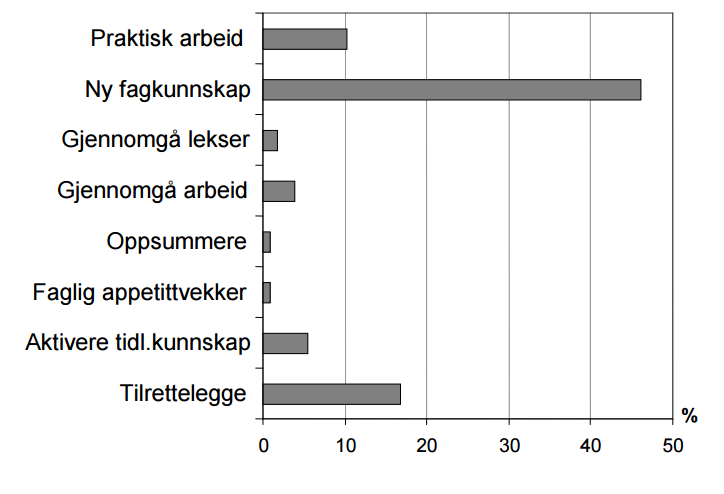
\includegraphics[scale = 0.6]{../figures/undervisnings_aktivitet.png}
\caption{Oversikt over naturfaglærernes undervisningstilbud til elevene fra PISA+ studie. Kilde: 
\protect\citeA{odeg10}.}
\label{fig:odeg10}
\end{figure}


\subsection*{Gruppe samtaler}
I helklassesamtalen ved starten av timen var det et fåtall elever som var aktive i lærer initiert 
diaglog. Dette var uheldig siden elevenes svakheter ble ikke tilstrekkelig avdekket. Gruppesamtalene 
viste seg å være en god plattform for å avdekke hull og svakheter i elevenes begrepsbruk. I den 
forbindelse ble tokolonnenotatet tatt i bruk (se vedlegg: \ref{sec:tokolonnenotat}).
\newline
\newline
I tokolonnenotatøvelsen viste noen grupper akkumulative tendenser. Det vil si at elevene 
var villig til å akseptere hverandres bidrag uten å stille kritiske spørsmål og fremsette
alternative forklaringer. Når elevene deretter ble fordelt i andre grupper og prøvde å
fremstille begrepene, viste noen elever svak forståelse. I blant ble begrepene fremstilt
overfladisk, og for noen elever ble deres svakheter om temaene avdekket.
\newline
\newline
En viktig del av den sosiale utprøvingen av ideer og begreper innebærer å sammenlikne egne 
forestillinger med andres forestillinger i tillegg til naturvitenskapens forklaringer 
(\citeNP{odeg10}; \citeNP{dals94}). Bruken av tokolonnenotatet i første timen 
\newline
\newline
Gode fagsentrerte samtaler mellom elever (eller faglige samtaler med lærer) hvor elever bruker egne 
erfaringer og språket for å oppnå faglig forståelse hjelper til å skape bro mellom praksis og teori 
(\citeNP{odeg10}).
\newline
\newline
Evnen til abstrahering henger ifølge Vygotsky (\citeNP[s. 127]{bta98}) med begrepsundervisning, som en
form for vitenskapeliggjøring av hverdagsbegreper. Hvis elever ikke har god begrepsforståelse
kan de ende opp med å bruke naturvitenskapelige begreper i feil kontekst og danne feil 
forbindelser med begrepene. Dette avhenger av deres forkunnskaper. Ausubels kognitive bruer 
(\citeNP[s. 71]{math15}), hans teori om begrepslæring på høyere nivå og hvordan læreren best kan 
legge til rette for slik læring og bruk av begrepene,  handler om å danne forbindelser mellom 
undervisningsmateriell og relevante ideer i elevenes kognitive struktur.
\newline
\newline
Stillasbygging (\citeNP{bta98}; \citeNP[s. 71]{math15})
% Selv om kognitiv forståelse alltid vil være avgjørende viktig i naturfag, så kan vi her spørre om det ikke nettopp er økt evne til deltagelse som bør være 
% begrunnelsen for å utvikle elevenes begrepsforståelse. Fokuset på forståelse må derfor suppleres med vektlegging av lesing for at naturfaget skal forberede til 
% demokratisk deltagelse 
%\citeA[s. ~72]{kols09}

% Slike begreper må være forstått for å kunne ta del i diskusjoner og argumentasjon, og er dermed en del av en naturfaglig allmenndannelse. En slik 
% begrepsforståelse må ses i sammenheng med opplæring i lesing av slike tekster. Ellers kan det være vanskelig å bruke slik kunnskap i nye situasjoner. 
%\citeA[s. ~67]{roen15}


\end{document}